Go.JS~\cite{gojs} es una biblioteca de JavaScript para implementar editores gráficos dentro de interfaces web. GoJS facilita la implementación de tareas tales como definición de símbolos gráficos, gestión de paletas de símbolos, arrastrar y soltar (\emph{drag and drop}), copiar y pegar, edición de etiquetas de texto asociadas a símbolos gráficos, menús contextuales, función de deshacer o la gestión de eventos de ratón, entre muchos otros elementos.

Para ilustrar el funcionamiento de GoJS, a continuación se mostrará a modeo de ejemplo cómo crear un editor gráfico para diseñar unos pseudo diagramas de flujo compuestos por círculos y rectángulos interconectados por flechas. Dicho editor se muestra en la Figura~\ref{fig:gojssample}.

\begin{figure}[!tb]
	\centering
	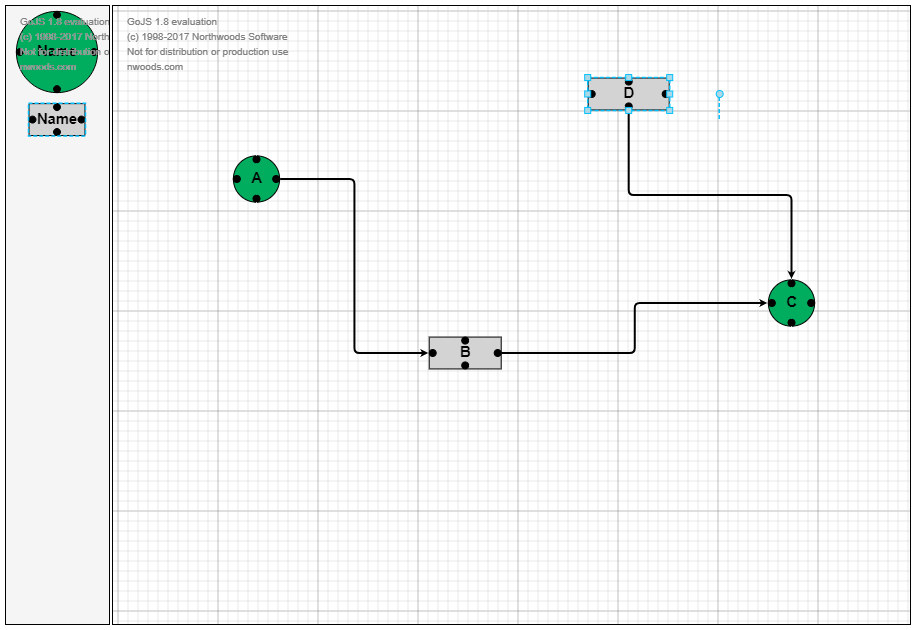
\includegraphics[width=\linewidth]{gojssample.png}
	\caption{Editor gráfico creado en GoJS}
    \label{fig:gojssample}
\end{figure}

Para comenzar, cabe destacar que, es necesario reservar dos secciones de la página HTML que lo contiene. Una sección albergará la paleta con los elementos gráficos del editor, que en este caso serán sólo el círculo y el rectángulo, y otra sección para el diagrama o lienzo sobre el que se depositarán los elementos gráficos.

A continuación, se debe realizar una serie de acciones a nivel de Javascript para proporcionar tanto a la paleta de dibujo como al área de dibujo del comportamiento deseado. En primer lugar, crearemos una variable \texttt{\$} que dé acceso al entorno GoJS. Esto se realiza mediante la llamada a la sentencia \texttt{make} de librería \emph{GraphObject} de GoJS (Figura~\ref{fig:asignacionDollar}, Línea~1).

\begin{figure}[!tb]
	\centering
	\begin{lstlisting}[language=JavaScript]
	var $ = go.GraphObject.make;
	\end{lstlisting}
	\caption{Asignación de la variable \texttt{\$}}
	\label{fig:asignacionDollar}
\end{figure}

Seguidamente, se personaliza la sección HTML reservada al diagrama, denominada \texttt{myDiagramDiv} (Figura~\ref{fig:creacionDiagrama}, Líneas~01-13), asignándole un \emph{grid} o cuadrícula de fondo (Figura~\ref{fig:creacionDiagrama}, Líneas~04-09), especificando los colores de las líneas de la cuadrícula (mediante la propiedad \emph{stroke}) y dándole la capacidad de poder arrastrar elementos sobre él (Figura~\ref{fig:creacionDiagrama}, Línea~10).

\begin{figure}[!tb]
	\centering
	\begin{lstlisting}[language=JavaScript]
	myDiagram =
		$(go.Diagram, "myDiagramDiv",
		{
			grid: $(go.Panel, "Grid",
				$(go.Shape, "LineH", { stroke: "lightgray", strokeWidth: 0.5 }),
				$(go.Shape, "LineH", { stroke: "gray", strokeWidth: 0.5, interval: 10 }),
				$(go.Shape, "LineV", { stroke: "lightgray", strokeWidth: 0.5 }),
				$(go.Shape, "LineV", { stroke: "gray", strokeWidth: 0.5, interval: 10 })
			),
			allowDrop: true,
		}
	);\end{lstlisting}
	\caption{Creación de un diagrama en GoJS}
	\label{fig:creacionDiagrama}
\end{figure}

A continuación deberemos definir lo que en GoJS se conoce como la \emph{plantilla de nodos} o \emph{node template}. Esta plantilla define el comportamiento genérico de todos los nodos que compondrán nuestro diagrama. Estos nodos, en nuestro caso, serán rectángulos y círculos. La Figura~\ref{fig:patronNodo} muestra cómo se crea el patrón que servirán de esqueleto para todos los nodos de nuestro diagrama. 

\begin{figure}[!tb]
	\centering
	\begin{lstlisting}[language=JavaScript]
	myDiagram.nodeTemplate =
		$(go.Node, "Spot",
		{ 
			locationSpot: go.Spot.Center 
		},
		new go.Binding("location").makeTwoWay(go.Point.stringify),
		{ 
			selectable: true, 
			selectionAdornmentTemplate: nodeSelectionAdornment 
		},
		{ 
			resizable: true, 
			resizeObjectName: "PANEL", 
			resizeAdornmentTemplate: nodeResizeAdornment 
		},
		{ 
			rotatable: true, 
			rotateAdornmentTemplate: nodeRotateAdornment 
		},
	
		$(go.Panel, "Auto",
		{ 
			name: "PANEL" 
		},
		$(go.Shape,
		{
			portId: "",
			fromLinkable: true, toLinkable: true, cursor: "pointer",
		},
		new go.Binding("figure"),
		new go.Binding("fill")),
		$(go.TextBlock,
		{
			maxSize: new go.Size(50, 50),
			editable: true
		},
		new go.Binding("text").makeTwoWay())
		)
	);\end{lstlisting}
\caption{Declaración del patrón del Nodo}
\label{fig:patronNodo}
\end{figure}

Para crear la definición un nodo lo primero es declarar el nodo con \texttt{\$(go.Node} (Figura~\ref{fig:patronNodo},~Línea~2).
A continuación, especificamos, mediante la definición de ciertas propiedades, cómo se comportará el nodo (Figura~\ref{fig:patronNodo}, Líneas~05-24). En nuestro caso, se indica que los nodo, con carácter general, podrán ser seleccionados, redimensionados y rotados (Figura~\ref{fig:patronNodo}, Líneas~05-07, respectivamente). Se establece que los nodos aparecerán localizados por defecto en el centro del diagrama en el momento de su creación (Figura~\ref{fig:patronNodo}, Línea~03).
Además, se indica que la propiedad \texttt{location}, que establece la posición del nodo, queda expuesta para su modificación desde el exterior (Figura~\ref{fig:patronNodo}, Línea~04).

Siempre que se crea un nodo, se reserva un espacio sobre el que se van a situar los diferentes elementos del nodo. En nuestro ejemplo, este espacio recibe el nombre de \emph{panel}(Figura~\ref{fig:patronNodo}, Línea~09). El panel actúa como contenedor de la figura (\emph{shape}) (Figura~\ref{fig:patronNodo}, Línea~11), que es la encargada de definir la forma del nodo. En nuestro caso, dicho panel podrá poseer diferentes formas (como serán el circulo y el rectángulo) y colores gracias a los \emph{bindings}, que son los que hacen que estas propiedades sean modificables programáticamente (Figura~\ref{fig:patronNodo}, Líneas~16-17). Además, cada nodo poseerá un identificador propio, denominado \emph{portId} (Figura~\ref{fig:patronNodo}, Línea~13) y todos los nodos pueden recibir conexiones tanto de entrado como de salida (\emph{toLinkable} y \texttt{fromLinkable}) (Figura~\ref{fig:patronNodo}, Línea~14). Por último, cada nodo poseerá una etiqueta de texto que permitirá especificar su nombre, el cual también puede ser modificado extenamente (Figura~\ref{fig:patronNodo}, Líneas~18-24).

Una vez definidas las propiedades básicas de un nodo, el siguiente paso es definir cómo enlazar dichos nodos. Para ello debemos definir dos elementos: \emph{puertos} y \emph{enlaces}. Los enlaces son los elementos que permiten conectar nodos, y los puertos de un nodo son los puntos de dicho nodo desde donde puede partir un enlace o a dónde puede llegar un enlace.  En la Figura~\ref{fig:gojssample}, estos puertos aparecen aparecen como unos círculos negros en los extremos de las figuras.

\begin{figure}[!tb]
	\centering
	\begin{lstlisting}[language=JavaScript]
	function makePort(name, spot) {
		return $(go.Shape, "Circle",
		{
			desiredSize: new go.Size(7, 7),
			alignment: spot,
			alignmentFocus: spot,
			portId: name,
			fromLinkable: true, toLinkable: true,
			cursor: "pointer"
		});
	}\end{lstlisting}
	\caption{Función MakePort}
	\label{fig:funcionMakeport}
\end{figure}
	
Para añadir puertos a los nodos se ha creado una función una función llamada \emph{makePort}, la cual se muestra en la Figura~\ref{fig:funcionMakeport}. Este fragmento de código define un puerto como una forma circular con un identificador (Figura~\ref{fig:funcionMakeport}, Línea~07), una posición (Figura~\ref{fig:funcionMakeport}, Líneas~05-06) y un tamaño (Figura~\ref{fig:funcionMakeport}, Línea~04). Finalmente, usando esta función, añadimos cuatro llamadas a a misma al final de la plantilla de nodos, con el objeto de crear un puerto a cada lado del eje de cada nodo (Figura~\ref{fig:patronNodoFinal}, Línea~04).

\begin{figure}[!tb]
	\centering
	\begin{lstlisting}[language=JavaScript]
	myDiagram.nodeTemplate =
		$(go.Node, "Spot",
		{ locationSpot: go.Spot.Center },
        ...
		makePort("T", go.Spot.Top),
		makePort("L", go.Spot.Left),
		makePort("R", go.Spot.Right),
		makePort("B", go.Spot.Bottom)
	);\end{lstlisting}
	\caption{Patrón Nodo con Puertos}
	\label{fig:patronNodoFinal}
\end{figure}

Una vez definidos los puertos, especificamos cómo se comportarán los enlaces entre nodos (Figura~\ref{fig:patronlink}). En nuestro caso, se declara que los enlaces irán de un nodo principal \texttt{isPanelMain} a uno secundario,  se efine el grosor del enlace y se establece que el enlace poseerá una flecha al final del mismo (\emph{toArrow: "Standard"}).

\begin{figure}[!tb]
	\centering
	\begin{lstlisting}[language=JavaScript]
	myDiagram.linkTemplate =
		$(go.Link,
			$(go.Shape,
			{ isPanelMain: true, strokeWidth: 2 }),
			$(go.Shape,
			{ toArrow: "Standard", stroke: null }
		)
	)\end{lstlisting}
\caption{Declaración del patrón del Link}
\label{fig:patronlink}
\end{figure}


\begin{figure}[!tb]
	\centering
\begin{lstlisting}[language=JavaScript]
myPalette =
	$(go.Palette, "myPaletteDiv",
	{
		nodeTemplateMap: myDiagram.nodeTemplateMap,
		model: new go.GraphLinksModel([
			{ 
				text: "Name", 
				figure: "Circle", 
				fill: "#00AD5F" 
			},
			{ 
				text: "Name", 
				figure: "Rectangle", 
				fill: "lightgray" 
			}
			])
		}
);\end{lstlisting}
\caption{Creación de la Paleta de Nodos}
\label{fig:paletaNodos}
\end{figure}

Por último, se procede a crear la paleta que contendrá los círculos y los rectángulos, tal como se muestra en la Figura~\ref{fig:paletaNodos}. Como se puede observar, la paleta se sitúa sobre una sección HTML denominada \emph{myPalleteDiv} (Figura~\ref{fig:paletaNodos}, Línea~XX), la cual fue reservada con anterioridad. Para la definición de los nodos que estarán dentro de la paleta se utiliza el mismo patrón e nodos creado con anterioridad (Figura~\ref{fig:paletaNodos}). Finalmente, por último, se declara el \emph{modelo}, que es el conjunto de figuras concretas que poseerá dicha paleta. Para crear los elementos del modelo, se instancia la plantilla de nodos y se cambian sus propiedades con objeto de crear objetos diferentes. En nuestro caso, creamos círculo de color verde (Figura~\ref{fig:paletaNodos}, Línea~06) y rectángulos de color gris (Figura~\ref{fig:paletaNodos}, Línea~07), ambos con \texttt{Name} como nombre por defecto, el cual podrá ser luego editado.

Una vez definidos estos elementos, nuestro editor gráfico queda implementado, y GoJS se encargará de dibujar la paleta y el diagrama, así como, de pintar los elementos sobre el área de dibujo cuando éstos sean seleccionados en la paleta, permitiendo arrastrarlos, redimensionarlos o renombrarlos, entre otras funciones.